  \documentclass{article}
\usepackage{pst-eucl}
\usepackage{changepage, amsmath, amssymb, pgfplots, tikz}
\usetikzlibrary{fit,positioning}
\usepgfplotslibrary{groupplots}
\usepackage[utf8]{inputenc}
\psset{PointName=none,PointSymbol=none}
\usetikzlibrary{arrows.meta}	
\usetikzlibrary{calc,patterns,angles,quotes}
\pgfplotsset{compat=1.16}
\usetikzlibrary{arrows.meta}
\usepackage{fullpage}
\usepackage{xparse,array}
\usetikzlibrary{circuits.ee.IEC}
\usepackage{ulem}
\usepackage{mathtools}
\usepackage{tikz}
\usetikzlibrary{tikzmark,calc}
\usepackage{geometry,graphicx}				% Paquetes adicionales.
\usepackage{subcaption,array}
\usepackage{multicol,multirow}
\usepackage{mathtools}
\usepackage{circuitikz,siunitx}
\usetikzlibrary{angles}
\usepackage{xcolor}
\usetikzlibrary{circuits.ee.IEC}
\usepackage[colorlinks=true, urlcolor=mypurple, linkcolor=myamber]{hyperref}
\usetikzlibrary{trees}
\usepackage[dvipsnames]{xcolor}
\usepackage{darkmode}
\enabledarkmode
\usepackage{framed} % or, "mdframed"
\usepackage{fancyhdr}
\usepackage{fontawesome}
\pagestyle{fancy}
\usepackage[framed]{ntheorem}
\usepackage{lmodern}
\usepackage{tabularx}
\usepackage{microtype}
\setlength{\columnsep}{1.5cm}
\setlength{\columnseprule}{0.4pt}
\usepackage{multicol}
\usetikzlibrary{arrows, shapes.gates.logic.US, calc}
\usetikzlibrary{calc,arrows.meta}
\usepackage[most]{tcolorbox}
\definecolor{p1}{HTML}{caf0f8}
\definecolor{p2}{HTML}{ade8f4}
\definecolor{p3}{HTML}{90e0ef}
\definecolor{p4}{HTML}{48cae4}
\definecolor{p5}{HTML}{00b4d8}
\definecolor{p6}{HTML}{0096c7}
\definecolor{p7}{HTML}{0077b6}
\definecolor{p8}{HTML}{023e8a}
\definecolor{p9}{HTML}{03045e}
\usepackage{multicol}
\usetikzlibrary {arrows.meta,graphs,shapes.misc}
\usetikzlibrary {positioning}
\usepackage{colortbl}
\colorlet{xcol}{blue!60!black}
\usepackage{capt-of}
\definecolor{myred}{HTML}{f44336}
\definecolor{mypink}{HTML}{e81e63}
\definecolor{mypurple}{HTML}{9c27b0}
\definecolor{mydeeppurple}{HTML}{673ab7}
\definecolor{myindigo}{HTML}{3f51b5}
\definecolor{myblue}{HTML}{2196f3}
\definecolor{mylightblue}{HTML}{03a9f4}
\definecolor{mycyan}{HTML}{00bcd4}
\definecolor{myteal}{HTML}{009688}
\definecolor{mygreen}{HTML}{4caf50}
\definecolor{mylightgreen}{HTML}{8bc34a}
\definecolor{mylime}{HTML}{cddc39}
\definecolor{myyellow}{HTML}{ffeb3b}
\definecolor{myamber}{HTML}{ffc107}
\definecolor{myorange}{HTML}{ff9800}
\definecolor{mydeeporange}{HTML}{ff5722}
\definecolor{mybrown}{HTML}{795548}
\definecolor{mygray}{HTML}{9e9e9e}
\definecolor{mybluegray}{HTML}{607d8b}
\definecolor{pag}{HTML}{293133}
\usepackage[labelformat=empty]{caption}
\usepackage{mdframed}
\newtcolorbox{qq}[2][]{%
	boxrule=0.75pt,
	sharp corners,  % Square edges
	colframe=white,  % Set the color of the outline
	colback=pag,  % Set the color of the fill
	coltext=white,
	#1,
}
\usepackage[framed]{ntheorem}
\newframedtheorem{frm-thm}{Theorem}

%portrail

\title{Análisis Matemático I}
\date{\today}
\author{Alejandro Ceccheto}
\begin{document}
	\maketitle
	\pagebreak
	
	\section{Teoría}


\vspace{0.5cm}
\begin{center}
	\begin{framed}
		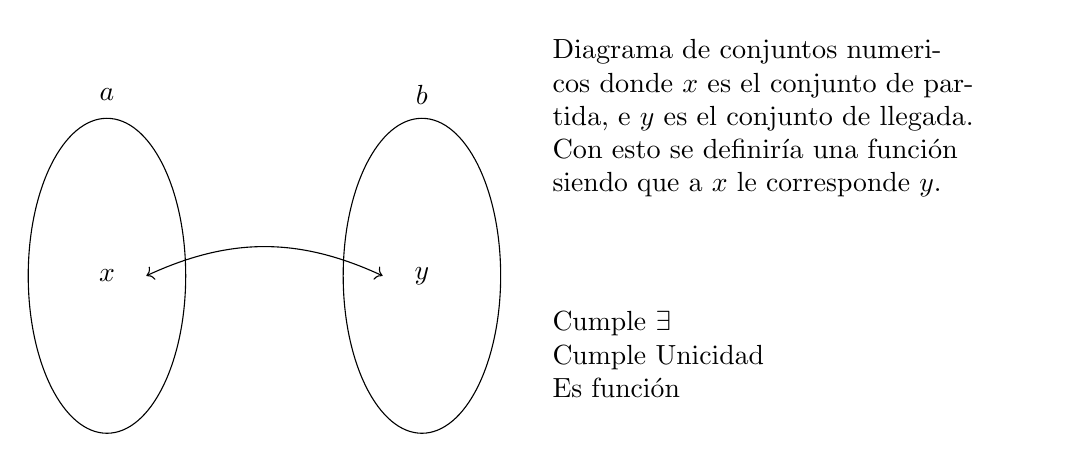
\begin{tikzpicture}
		\node at (0,2.3) {$a$};
		\node at (4,2.3) {$b$};
		\draw (0,0) ellipse [x radius = 1cm, y radius = 2cm];
		\draw (4,0) ellipse [x radius = 1cm, y radius = 2cm];
		\draw (0,0) node {$x$};
		\draw (4,0) node {$y$};
		\draw[<->] (0.5,0) to [bend left=25] (3.5,0);
		\draw ;
		\node at (4.5,2) [right=1cm,text width=6cm,rounded corners,inner sep=1ex,]
		{ Diagrama de conjuntos numericos donde $x$ es el conjunto de partida, e $y$ es el conjunto de llegada. \linebreak
			Con esto se definiría una función siendo que a $x$ le corresponde $y$.
		};
		\node  at (4.5,-1)[right=1cm,text width=6cm,rounded corners,inner sep=1ex,]{Cumple $\exists$ \\
		          Cumple Unicidad \\
		          Es función};
	\end{tikzpicture}
	\end{framed}
\end{center}
	

\begin{center}
	\begin{framed}
		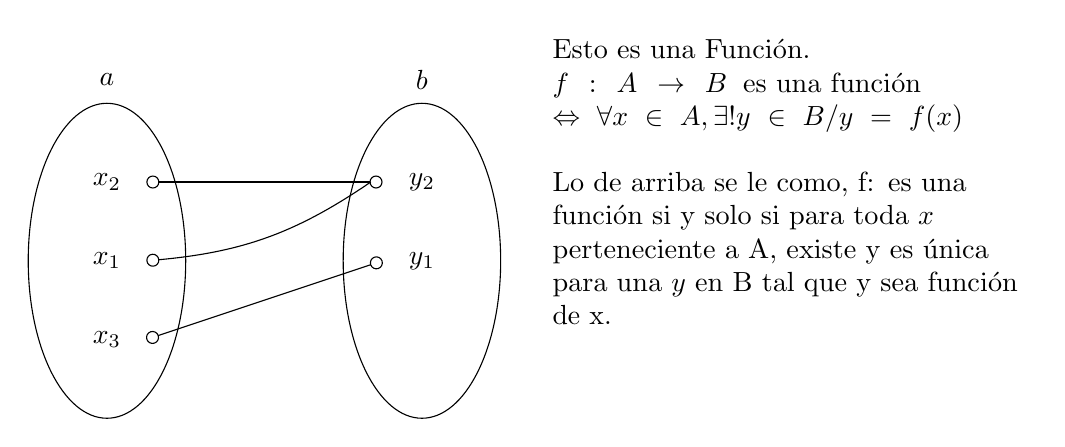
\begin{tikzpicture}
			\draw (0,0) ellipse [x radius = 1cm, y radius = 2cm];
			\draw (4,0) ellipse [x radius = 1cm, y radius = 2cm];
			\draw (0,0) node {$x_1$};
			\draw (0,1) node {$x_2$};
			\draw (0,-1) node {$x_3$};
			\draw (4,0) node {$y_1$};
			\draw (4,1) node {$y_2$};
			
			
			\draw[o-o] (0.5,-1) to (3.5,0);
			\draw[o-] (0.5,0)  to [bend right=15]  (3.35,1);
			\draw[o-o] (0.5,1)  to (3.5,1);
			\node at (4.5,1) [right=1cm,text width=6cm,rounded corners,inner sep=1ex,]
			{Esto es una Función. \linebreak
			$f : A \rightarrow B \hspace{0.2cm} $es una función$ \hspace{0.2cm} $\linebreak$ \Leftrightarrow   \forall x \in A, \exists! y \in B / y = f(x) $ \linebreak
			
			
			Lo de arriba se le como, f: es una función si y solo si para toda $x$ perteneciente a A, existe y es única para una $y$ en B tal que y sea función de x.};
			\node at (0,2.3) {$a$};
			\node at (4,2.3) {$b$};
		\end{tikzpicture}
	\end{framed}
\end{center}

	
\begin{center}
	\begin{framed}
		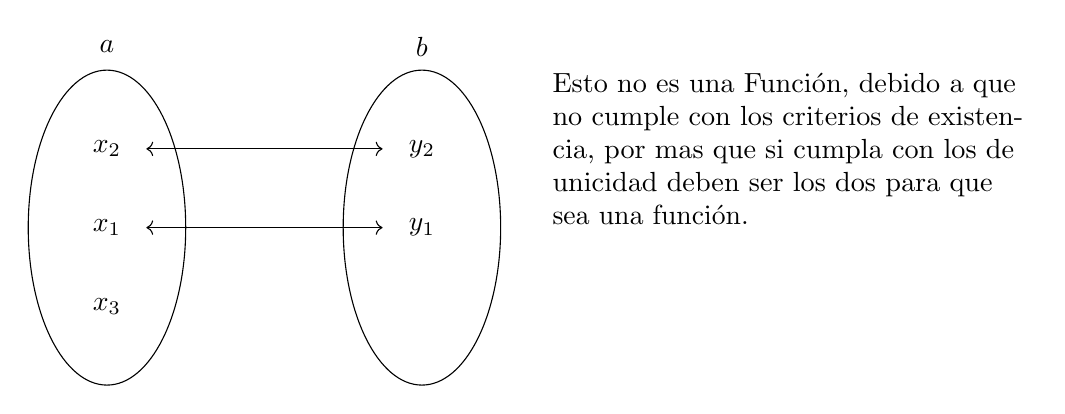
\begin{tikzpicture}
			\node at (0,2.3) {$a$};
			\node at (4,2.3) {$b$};
			\draw (0,0) ellipse [x radius = 1cm, y radius = 2cm];
			\draw (4,0) ellipse [x radius = 1cm, y radius = 2cm];
			\draw (0,0) node {$x_1$};
			\draw (0,1) node {$x_2$};
			\draw (0,-1)node {$x_3$};
			\draw (4,0) node {$y_1$};
			\draw (4,1) node {$y_2$};
			
			\draw[<->] (0.5,1) to (3.5,1);
			\draw[<->] (0.5,0) to  (3.5,0);
			
			\node at (4.5,1) [right=1cm,text width=6cm,rounded corners,inner sep=1ex,]
			{Esto no es una Función, debido a que no cumple con los criterios de existencia, por mas que si cumpla con los de unicidad deben ser los dos para que sea una función.};
		\end{tikzpicture}
	\end{framed}
\end{center}	

\section{Ejemplo.}
\vspace{0.3cm}
Como ejemplo se utilizo una función raíz cuadrada de lo mas conocida, generalmente es utilizada para explicar el tema.

	\begin{framed}
		\begin{equation*}
			\sqrt{x-1}
		\end{equation*}
		\begin{center}
			\begin{tikzpicture}[scale=0.9]
				\begin{axis}[axis lines=center, minor tick num=3]
					\addplot[samples=80, smooth, thick, domain=0:10]
					{sqrt(x-1)};
					
				\end{axis}
			\end{tikzpicture}
		\end{center}
	\end{framed}
	
	\subsubsection{Desarrollo.}
	
	
	$h: D_h \rightarrow \mathbb{R} / h(x) = \sqrt{x-1}$
	
	\begin{center}
		\begin{equation}
			\sqrt{x-1} \rightarrow x \geq 0
		\end{equation}
		\begin{equation}
			x-1 \geq 0 
		\end{equation}
		\begin{equation}
			x \geq 1
		\end{equation}
		\begin{equation}
			D_h = [1;+\infty) \hspace{0.2cm} \neq \hspace{0.2cm} \mathbb{R}^+ - \left\{1\right\} \footnote{Siendo la primera la forma correcta de como se expresa un segmento en una recta real, la segunda forma es la equivocada}
		\end{equation}
		\begin{equation*}
			Imgf = \mathbb{R}^+ \Leftrightarrow [0;+\infty]
		\end{equation*} 
		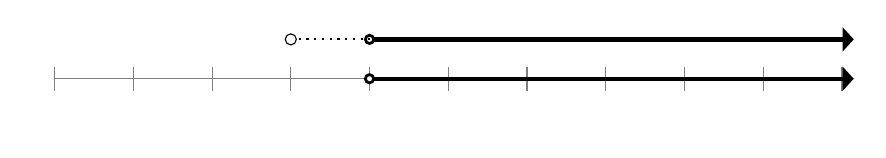
\begin{tikzpicture}[
			line/.style = {draw, ultra thick, shorten <=-2pt},
			La/.style = {line, shorten >=-2pt,
				{Circle[length=4pt, line width=1pt]}-{Circle[length=4pt,line width=1pt, fill=white]}},
			Lb/.style = {line, shorten >=-2pt,
				{Circle[length=4pt, line width=1pt, fill=white]}-{Circle[length=4pt, line width=1pt]}},
			Lc/.style = {line,
				{Circle[length=4pt, line width=1pt, fill=white]}-{Triangle[length=4pt, line width=1pt]}},
			Lq/.style = {line, shorten >=-2pt,
				{Circle[length=4pt, line width=1pt, fill=white]}-{Circle[length=4pt,line width=1pt, fill=white]}},
			Ld/.style = {line, shorten >=-2pt,
				{Circle[length=4pt, line width=1pt]}-{Circle[length=4pt, line width=1pt]}},
			Ldo/.style = {dotted, shorten >=-2pt,
				{Circle[length=4pt, line width=1pt]}-{Circle[length=4pt,line width=1pt, fill=white]}},	
			]
		
					\draw[gray] (-3,0) -- (7,0);    % <---
					\foreach \i in {-3,-2,...,7} % numbers on line
					\draw[gray] (\i,0.15) -- ++ (0,-0.3)    % <---
					node[below,text=white] {$\i$}; % tick and their labels
					
					\draw[Lc] (1,0) to (7.15,0) ;
					\draw[Lc] (1,0.5) to (7.15,0.5);
					\draw[dotted, thick] (0,0.5) to (1,0.5);
					\draw[fill=white] (0,0.5) circle[radius = 2pt];
					
		\end{tikzpicture}
	\end{center}
	
	
	\pagebreak
	
	
	\section{Ejemplo}
	
		\begin{framed}
			\begin{center}
				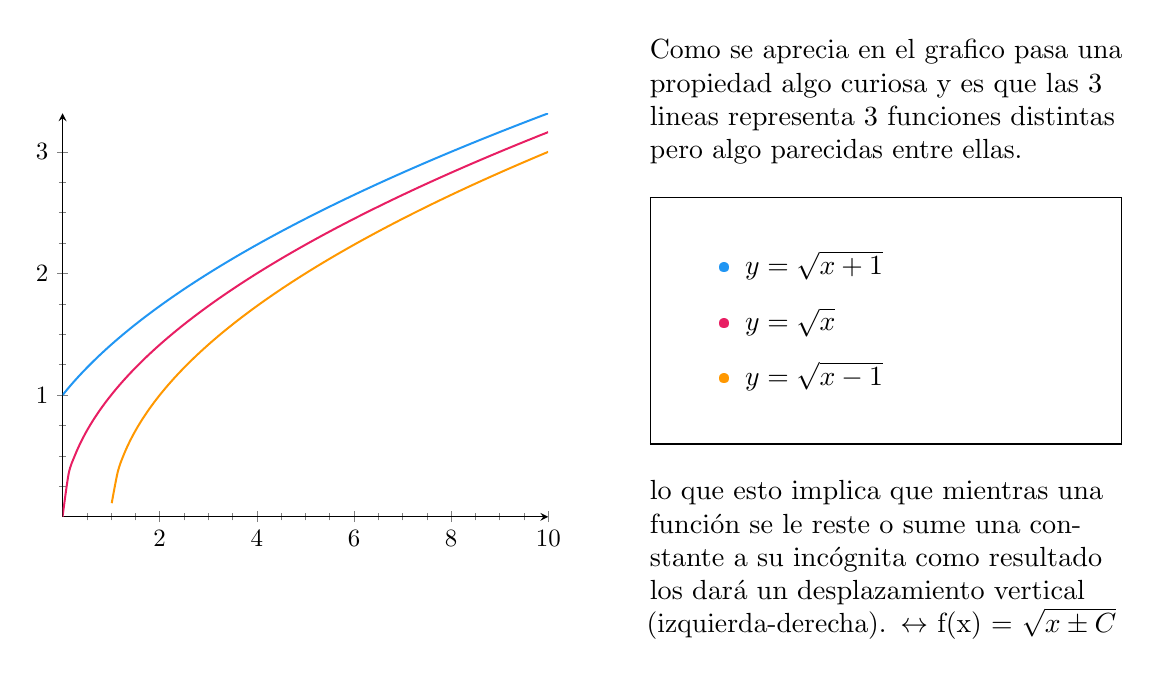
\begin{tikzpicture}[scale=0.9]
					\begin{axis}[axis lines=center, minor tick num=3]
						\addplot[samples=80, smooth, thick, domain=0:10, color=myblue]
						{sqrt(x+1)};
						\addplot[samples=80, smooth, thick, domain=0:10, color=mypink] 
						{sqrt(x)};
						\addplot[samples=80, smooth, thick, domain=0:10, color=myorange] 
						{sqrt(x-1)};
					\end{axis}
						\node at (7,4.-1.5) [right=1cm,text width=6cm,rounded corners,inner sep=1ex,]
					{Como se aprecia en el grafico pasa una propiedad algo curiosa y es que las 3 lineas representa 3 funciones distintas pero algo parecidas entre ellas.\\
					 \begin{framed}
					 	\begin{itemize}
					 		\item[\textcolor{myblue}{\textbullet}] $y=\sqrt{x+1}$ \\
					 		\item[\textcolor{mypink}{\textbullet}] $y=\sqrt{x}$ \\
					 		\item[\textcolor{myorange}{\textbullet}] $y=\sqrt{x-1}$
					 	\end{itemize}
					 \end{framed}
					 lo que esto implica que mientras una función se le reste o sume una constante a su incógnita como resultado los dará un desplazamiento vertical (izquierda-derecha). $\leftrightarrow$ f(x) = $\sqrt{x \pm C}$
					};
				\end{tikzpicture}
			\end{center}
		\end{framed}
		\begin{framed}
			\begin{center}
				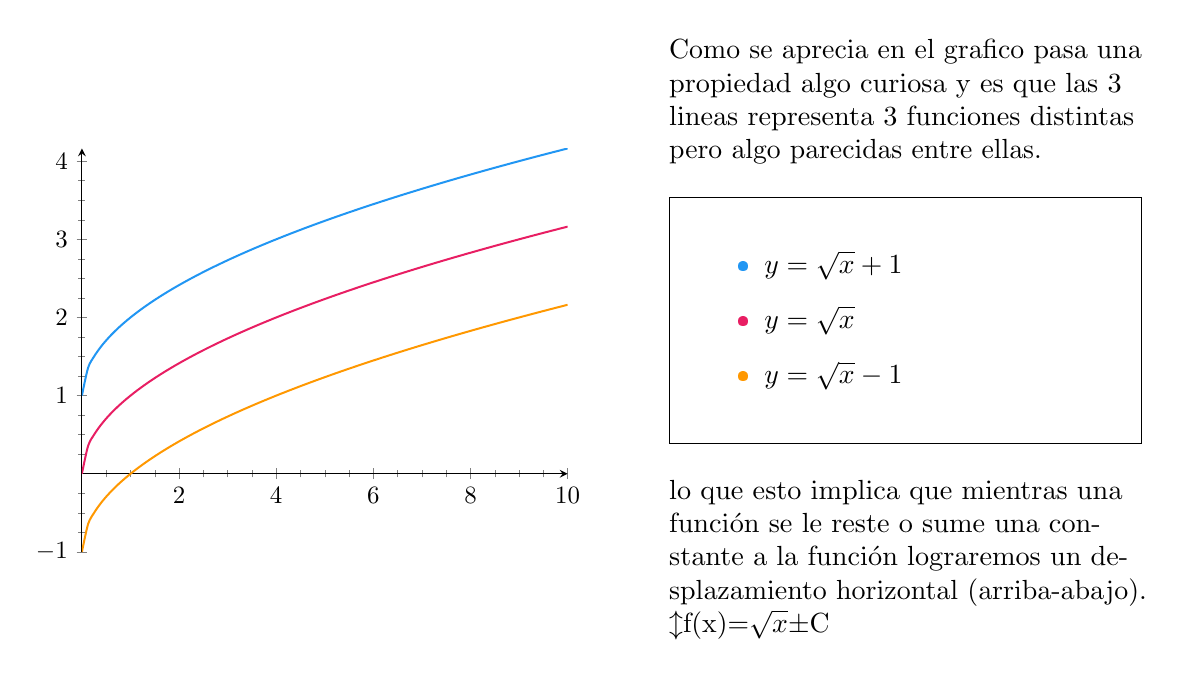
\begin{tikzpicture}[scale=0.9]
					\begin{axis}[axis lines=center, minor tick num=3]
						\addplot[samples=80, smooth, thick, domain=0:10, color=myblue]
						{sqrt(x)+1};
						\addplot[samples=80, smooth, thick, domain=0:10, color=mypink] 
						{sqrt(x)};
						\addplot[samples=80, smooth, thick, domain=0:10, color=myorange] 
						{sqrt(x)-1};
					\end{axis}
					\node at (7,4.-1) [right=1cm,text width=6cm,rounded corners,inner sep=1ex,]
					{Como se aprecia en el grafico pasa una propiedad algo curiosa y es que las 3 lineas representa 3 funciones distintas pero algo parecidas entre ellas.\\
						\begin{framed}
							\begin{itemize}
								\item[\textcolor{myblue}{\textbullet}] $y=\sqrt{x}+1$ \\
								\item[\textcolor{mypink}{\textbullet}] $y=\sqrt{x}$ \\
								\item[\textcolor{myorange}{\textbullet}] $y=\sqrt{x}-1$
							\end{itemize}
						\end{framed}
						lo que esto implica que mientras una función se le reste o sume una constante a la función lograremos un desplazamiento horizontal (arriba-abajo). $\updownarrow$f(x)=$\sqrt{x}$$\pm$C
					};
				\end{tikzpicture}
			\end{center}
		\end{framed}
		
		\pagebreak
		
		\section{Función Lineal.}
	\begin{framed}
		\begin{equation*}
			y=mx+b
		\end{equation*}
		\begin{center}
					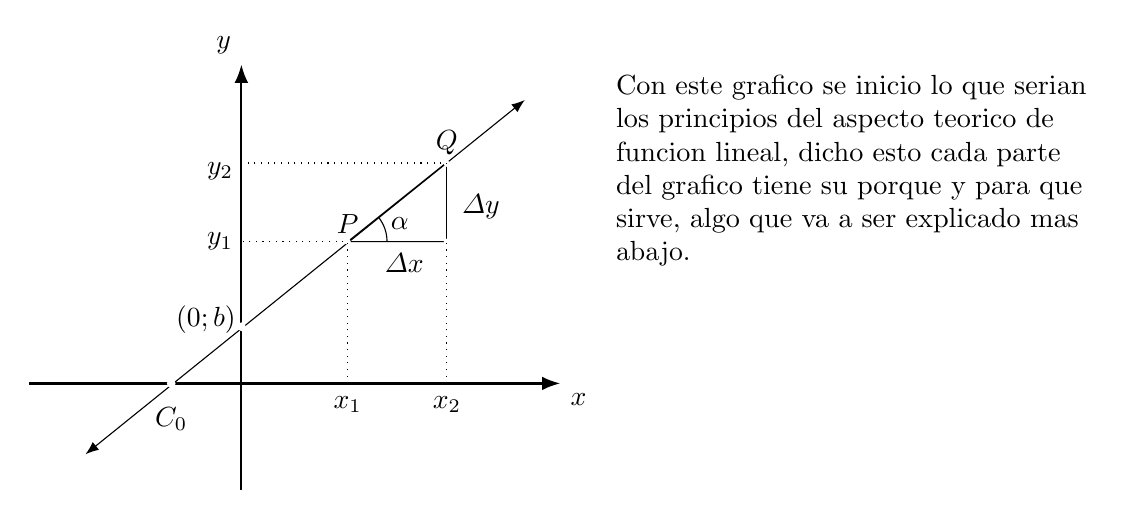
\begin{tikzpicture}[scale=0.9, >=Latex]
						%\draw[step=1cm,gray,very thin] (-1,-1) grid (6,6);
					\draw[thick,->] (-3,0) -- (4.5,0) node[anchor=north west] {$x$};
					\draw[thick,->] (0,-1.5) -- (0,4.5) node[anchor=south east] {$y$};
					\foreach \x in {}
					\draw (\x cm,1pt) -- (\x cm,-1pt) node[anchor=north] {$\x$};
					\foreach \y in {}
					\draw (1pt,\y cm) -- (-1pt,\y cm) node[anchor=east] {$\y$};
					\draw[<->] (-2.2,-1) -- (4,4);
					\draw (2.9,2) -- (2.9,3.1);
					\node at (3.38,2.5){$\varDelta y$};
					\node at (2.3,1.7){$\varDelta x$};
					\draw (2.9,2) coordinate (A) -- (1.5,2) coordinate (B) -- (2.9,3.12) coordinate (C)
					pic ["$\alpha$", draw, angle eccentricity=1.4] {angle};
					\filldraw[white] (2.9,2) circle [radius=1pt]
					                 (1.5,2) circle [radius=1pt]
					                 (2.9,3.1) circle [radius=1pt]
					                 (0,0.8) circle [radius=1.5pt]
					                 (-0.99,0) circle [radius=1.5pt];
					\draw[dotted] (1.5,0) -- (1.5,2) -- (0,2) ;
					\draw[dotted] (2.9,0) -- (2.9,3.11) -- (0,3.11);
					\node at (-0.3,3) {$y_2$};
					\node at (2.9,-0.3) {$x_2$};
					\node at (1.5,-0.3) {$x_1$};
					\node at (-0.3,2) {$y_1$};
					\node at (1.5,2.25) {$P$};
					\node at (2.9,3.4) {$Q$};
					\node at (-0.5,0.9) {$(0;b)$};
					\node at (-0.99,-0.5) {$C_0$};
					\node at (4,4.-1) [right=1cm,text width=6cm,rounded corners,inner sep=1ex,]
					{Con este grafico se inicio lo que serian los principios del aspecto teorico de funcion lineal, dicho esto cada parte del grafico tiene su porque y para que sirve, algo que va a ser explicado mas abajo.};
				\end{tikzpicture}
		\end{center}
	\end{framed}
	
	A continuación, vamos a detallar todo lo que se encuentra en el grafico explicando que es cada segmento del mismo, para un mayor entendimiento.
	
	Para empezar lo mas importante es identificar las partes notables de una función lineal explicita/natural $y=mx+b$ y es igual a m por x mas b.
	Esto es así siempre para una función lineal, lo que nos importa es ubicar que es y, que es m, que es x u que es b, esto suele ser al principio algo tedioso pero a la larga se memoriza como cualquier cosa y sale solo. \\
	Empezando por el princio $y = f(x)$, es la variable dependiente de $x$, siempre va a ser asi, indica la función, y como se ve, decir $y = mx+b$ es lo mismo que decir $f(x) = mx+b$.
	\begin{center}
		\section*{Ejemplo.}
		\begin{equation*}
			y = mx+b \equiv f(x)=mx+b
		\end{equation*}
	\end{center}
	
	$C_0$ es el punto donde la función corta con el eje de las abscisas ó $x$.
	\begin{center}
		\begin{equation*}
			C_0 = f(x) = 0 = C_0 = {x\in Df / f(x) = 0}
		\end{equation*}
	\end{center} 
	Lo escrito arriba, en lenguaje coloquial define que es el conjunto de ceros, en síntesis dice que el conjunto de cero es cuando la función es igual a cero en donde x pertenece al dominio de la función tal que la función es igual a cero.
	\pagebreak
	\section{Función Lineal.}
	\vspace{5pt}
	$C\uparrow$ es el conjunto de positividad de una función, determina donde una funcion esta por encima del eje de las abscisas ó $x$.
	\begin{center}
		\begin{equation*}
			C\uparrow = f(x) > 0 = C+ = {x\in Df / f(x) > 0} \hspace{1cm} C\uparrow=[X_0;+\infty]
		\end{equation*}
	\end{center}
	Conjunto de positividad es igual a la función cuando es mayor a 0 en donde $x$ pertenece al dominio de la función tal que la función es mayor a cero. \\
	
	\vspace{1cm}
	
	
	$C\downarrow$ es el conjunto de negatividad, siendo el opositor del de positividad, este se da cuando la función es menor que 0, por lo tanto da como resultado todos los puntos donde la función es negativa.
	
	\begin{center}
		\begin{equation*}
			C\downarrow = f(x) < 0 = {x\in Df / f(x) < 0} \hspace{1cm} C\downarrow=[X_0;-\infty]
		\end{equation*}
	\end{center}
	Conjunto de negatividad es igual a la funcion menor que 0 en donde x pertenece al Dominio de la función tal que la función es menor que cero. 
	
	\vspace{1cm}
	
	$\varDelta x / \varDelta y$ = diferencial $x$ y diferencial $y$ son las bases que sentaron la forma en la que se puede calcular la pendiente de una función lineal tal que la pendiente es la diferencia entre estas dos.
	
	\begin{equation*}
		\varDelta x = x_2 - x_1 \hspace{1cm} \varDelta y = y_2 - y_1 
	\end{equation*} 
	esto es debido a que se resta los valores de cada coordenada de los pares ordenados entre si.
	\begin{equation*}
		m = \frac{\varDelta y}{\varDelta x }\hspace{0.5cm}\equiv\hspace{0.5cm} m = \frac{y_2 - y_1}{x_2 - x_1}
	\end{equation*}
	
	\section*{Ecuación de Segmento.}
	
	Otra formula que puede ser de mucha ayuda e la ecuación para sacar el segmento por el que pasa por $x$ e $y$ de la función, por ejemplo.
	
	Siendo esta la ecuación de la recta explicita.
	\begin{equation*}
		\frac{-m}{b}x + \frac{y}{b} = 1
	\end{equation*}
	\pagebreak
	\section{Función Lineal.}
	podemos deducir que: 
	\begin{center}
		\begin{flalign*}
		& y = \frac{2}{3}x -4&\\
		& y -\frac{2}{3}x = -4&\\
		& \frac{y}{-4} + \frac{2x}{4 \cdot 3}= 1&\\
		& \frac{y}{-4} + \frac{x}{6} = 1
	\end{flalign*}
	\end{center}
	
	siendo -4 y 6 dos valores notables que si graficaramos la función darian exactamente en la raiz de la funcion $C_0$ y la O.O (ordenada al origen).
	
	\begin{framed}
		\begin{center}
		\begin{tikzpicture}[scale=0.9]
			\begin{axis}[axis lines=center, minor tick num=3]
				\addplot[samples=80, smooth, thick, domain=0:10, color=myblue]
				{2/3*x-4};
			\end{axis}
			\node at (6,3) [right=1cm,text width=6cm,rounded corners,inner sep=1ex,]
			{Como se ve en el grafico, el $-4$ es igual a la ordenada a la origen y el 6 la Raiz o $C_0$.};
		\end{tikzpicture}
	\end{center}
	\end{framed}
	
	
	
	
	
	
\end{document}